\section{Introduction}
\textbf{support vector machine} (SVM, also support vector networks) is a kind of binary classification models of supervised learning. Given a set of training examples, each marked as belonging to one or the other of two categories, an SVM training algorithm builds a model that assigns new examples to one category or the other, making it a non-probabilistic binary classifier.
\par From simple to complex,there are 3 levels of SVM,which are linear SVM in linearly separable case,linear SVM and non-linear SVM.
\begin{itemize}
  \item linear SVM in linearly separable case: while training data is linearly separable,we can use hard margin maximization algorithms to learn a binary linear classification.
  \item linear SVM: while training data is approximately linearly separable,we can use soft margin maximization algorithms to learn a binary linear classification.
  \item non-linear SVM: while training data isn't linearly separable,we can use kernel methods with soft margin maximization algorithms to learn a binary non-linear classifier.
\end{itemize}


\section{Linear SVM in linearly separable case}
\paragraph{Linearly separable} Let $\displaystyle X_{0}$ and $\displaystyle X_{1}$  be two sets of points in an n-dimensional Euclidean space.Then $\displaystyle X_{0}$ and $\displaystyle X_{1}$ are linearly separable if there exists an $n$-dimensional real vector $\omega$ and a real value b, such that every point $\displaystyle x\in X_{0}$ satisfies $\displaystyle\omega\cdot x+b>0$ and every point $\displaystyle x\in X_{1}$ satisfies $\displaystyle \omega\cdot x+b<0$.
\\
\\We are given a training dataset of $\displaystyle N$ points of the form
$$(x_{1},y_{1}),\cdots,(x_{N},y_{N})$$
where $\displaystyle x_{i}\in \mathbf{R}^n,y_{i}\in \{-1,1\}$.$\displaystyle y_{i}$ is a label that indicates which category $\displaystyle x_{i}$ belongs  to.And we suppose that our training data is linearly separable.
\par We want to find the "maximum-margin hyperplane" that divides the group of points $x_{i}$ for which $\displaystyle y_{i}=1$ from the group of points for which $\displaystyle y_{i}=-1$, which is defined so that the distance between the hyperplane and the nearest point $\displaystyle x_{i}$ from either group is maximized.
\par Any hyperplane can be written as the set of points $\displaystyle x$ satisfying $\displaystyle \omega\cdot x+b=0$,where $\displaystyle \omega$ is the (not necessarily normalized) normal vector to the hyperplane.The parameter $\displaystyle\ \frac{b}{\|\omega\|}\ $ determines the offset of the hyperplane from the origin along the normal vector $\displaystyle\omega$.

\subsection{Hard margin}

If the training data are linearly separable, we can select two parallel hyperplanes that separate the two classes of data, so that the distance between them is as large as possible. The region bounded by these two hyperplanes is called the "margin", and the maximum-margin hyperplane is the hyperplane that lies halfway between them.
\noindent

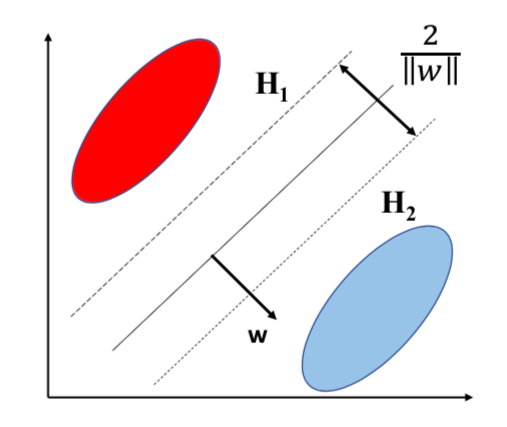
\includegraphics[height=5cm]{margin}

\paragraph{Functional margin} Given a training dataset $T$ and hyperplane $\displaystyle(\omega,b)$,we define the functional margin of hyperplane $\displaystyle(\omega,b)$ $w.r.t.$ data $\displaystyle(x_{i},y_{i})$ as
\begin{equation}
\widehat{\gamma_{i}}=y_{i}(\omega\cdot x_{i}+b)
\end{equation}
and can define the functional margin of hyperplane $\displaystyle(\omega,b)$ $w.r.t.$ dataset $T$ as
\begin{equation}
\widehat{\gamma}=\min_{i=1,\cdots,N}\widehat{\gamma_{i}}
\end{equation}

\paragraph{Geometric margin} Given a training dataset $T$ and hyperplane $(\omega,b)$,we define the geometric margin of hyperplane $(\omega,b)$ $w.r.t.$ data $(x_{i},y_{i})$ as
\begin{equation}
\displaystyle\gamma_{i}=\frac{\widehat{\gamma_{i}}}{\|\omega\|}
\end{equation}
and can define the functional margin of hyperplane $(\omega,b)$ $w.r.t.$ dataset $T$ as
\begin{equation}
\displaystyle\gamma=\min_{i=1,\cdots,N}\gamma_{i}=\frac{\widehat{\gamma}}{\|\omega\|}
\end{equation}
\\Notice that if we change $(\omega,b)$ into $(\lambda\omega,\lambda b)$,the hyperplane and geometric margin remain unchanged,but functional margin $\displaystyle\widehat{\gamma}$ changes into $\displaystyle\lambda\widehat{\gamma}$.In fact,what we want to maximize is geometric margin,but we can use the freedom of functional margin to simplify the optimization problem.

\subsection{Hard margin maximization method}

The basic idea of linear SVM is to maximize the geometric margin,and to find maximum margin classifier.The problem can be described as follows
\begin{equation}
 \begin{split}
  &\max_{\bm\omega,b}\ \ \gamma\\
  &s.t.\ \min\limits_{i=1,2,\cdots,N}\ y_{i}(\bm\omega\bm\cdot\bm x_{i}+b)>0\\
 \end{split}
\end{equation}
Notice two things below:
\begin{enumerate}
 \item $\gamma(\lambda\bm\omega,\lambda b)=\gamma(\bm\omega,b)$
 \item Given $(\bm\omega,b)$, there always exists a $\lambda$ such that $\widehat{\gamma}(\lambda\bm\omega,\lambda b)=1$
\end{enumerate}
So if we add an extra restraint $\ \widehat{\gamma}(\bm\omega,b)=1$, it won't affect the result of (5). Then problem (5) turns out to be
\begin{equation}
 \begin{split}
  &\max_{\omega,b}\ \ \frac{1}{\|\bm\omega\|}\\
  &s.t.\ \min\limits_{i=1,2,\cdots,N}\ y_{i}(\bm\omega\bm\cdot\bm x_{i}+b)=1\\
 \end{split}
\end{equation}
In order to change (6) into a convex problem, we expand constraint domain to a convex domain by adding points $(\bm\omega,b)$ which satisfies $\widehat{\gamma}(\bm\omega,b)>1$.
\\Suppose $\widehat{\gamma}(\bm\omega_{0},b_{0})>1$, take $\displaystyle\bm\omega_{1}=\frac{\bm\omega_{0}}{\widehat{\gamma_{0}}},\ b_{1}=\frac{b_{0}}{\widehat{\gamma_{0}}}$, we have $$\displaystyle\gamma(\bm\omega_{1},b_{1})=1,\ \ \frac{1}{\|\bm\omega_{1}\|}=\frac{\widehat{\gamma_{0}}}{\|\bm\omega_{0}\|}>\frac{1}{\|\bm\omega_{0}\|}$$.
So we can see that this operation won't affect the result of (6). Meanwhile, to maximize $\displaystyle\frac{1}{\|\bm\omega\|}$ is equally to minimize $\displaystyle\frac{1}{2}\|\bm\omega\|^2$, our problem can be finally written as following
\begin{equation}
 \begin{split}
  &\min_{\bm\omega,b}\ \frac{1}{2}\|\bm\omega\|^{2}\\
  &s.t.\ \ y_{i}(\bm\omega\bm\cdot\bm x_{i}+b)\geq 1,\ i=1,2,\cdots ,N
 \end{split}
\end{equation}

\begin{algorithm}
\caption{Hard margin maximization method}
\textbf{Input:} linearly separable dataset $T=\{(x_{1},y_{1}),\cdots,(x_{N},y_{N})\},x_{i}\in\chi=\textbf{R}^n ,y_{i}\in\Upsilon=\{-1,1\},i=1,2,\cdots,N\\$
\textbf{Output:} maximum margin hyperplane $(\omega,b)$ and classification decision function $f(x)=sign(\omega\cdot x+b)$
\begin{algorithmic}[1]
\State Solve problem (7),get optimal solution $(\omega^*,b^*)$
\State get maximum margin hyperplane $\omega^*\cdot x+b^*=0$ and classification decision function $f(x)=sign(\omega^*\cdot x+b)$
\end{algorithmic}
\end{algorithm}

\begin{theorem}
 If training dataset$T$ is linearly separable,the solution of problem (1) exists uniquely, in other words,the maximum margin hyperplane exists uniquely.
\end{theorem}

\paragraph{Support vector} If training dataset $T$ is linearly separable,then $x$ is a support vector precisely when $\ y(\omega\cdot x+b)=1$.

\subsection{Dual method}

In order to solve problem (7), we can consider it as a primal problem,use Lagrange duality theory to get its dual problem. And we can solve the dual problem to get the solution of the primal problem.

\paragraph{Remark} Here we'll introduce several conclusions in convex optimization programming before going further in dual method.
\\Consider a convex optimal problem:
\begin{equation}
\begin{split}
&\min_{x\in\textbf{R}^n} f(x)\\
&s.t.\ c_{i}(x)\leq 0,\ i=1,2,\cdots,k;\ h_{j}(x)=0,\ j=1,2,\cdots,l
\end{split}
\end{equation}
\\We call this problem a primal problem.Its generalized Lagrange function is
\begin{equation}
L(x,\alpha,\beta)=f(x)+\sum\limits_{i=1}^{k}\alpha_{i}c_{i}(x)+\sum\limits_{i=1}^{l}\beta_{j}h_{j}(x)
\end{equation}
Here,$x=(x^{(1)},x^{(2)},\cdots,x^{(n)})\in\ \mathbf{R}^n$,$\alpha,\beta$ is Lagrange multiplier,$\alpha_{i}\geq 0$.
\\Consider problem
\begin{equation}
d^*=\min\limits_{x}\max\limits_{\alpha,\beta;\alpha\geq 0}\ \ L(x,\alpha,\beta)
\end{equation}
We can easily prove that problem $(10)$ is equal to problem $(8)$.
Meanwhile,the dual problem of $(10)$ is defined as
\begin{equation}
p^*=\max\limits_{\alpha,\beta;\alpha\geq 0}\min\limits_{x}\ \ L(x,\alpha,\beta)
\end{equation}

we have following theorem.

\begin{theorem}[KKT]
 Suppose that $f(x)$ and $c_{i}(x)$ are convex functions, $h_{j}(x)$ is an affine function,meanwhile, inequality constraint $c_{i}(x)$ is strictly feasible, which means $\exists x,\ \forall i,\ c_{i}(x)<0$.
 \begin{itemize}
   \item $\exists\ x^*,\bm\alpha^*,\bm\beta^*$, such that $x^*$ is the solution of the primal problem $(7)$, $\bm\alpha^*,\bm\beta^*$ is the solution of the dual problem $(8)$,and $d^*=p^*=L(x^*,\bm\alpha^*,\bm\beta^*)$.
   \item $x^*$ is the solution of the primal problem $(7)$, $\bm\alpha^*,\bm\beta^*$ is the solution of the dual problem $(8)$ $iff$ $x^*,\bm\alpha^*,\bm\beta^*$ satisfy:
         \begin{equation}
	     \left\{
	     \begin{split}
	     &\nabla_{x} L(x^*,\bm \alpha^*, \bm \beta^*)&=0\\
         &\nabla_{\bm\alpha} L(x^*,\bm \alpha^*, \bm \beta^*)&=0\\
         &\nabla_{\bm\beta} L(x^*,\bm \alpha^*, \bm \beta^*)&=0\\
	     &\alpha_i^* c_i(x^*)&=0\\
	     & c_i(x^*)&\leq 0\\
	     &\alpha_i^* &\geq 0\\
	     &h_j(x^*) &= 0\\
	     \end{split}
	     \right.
	     \end{equation}
 \end{itemize}
\end{theorem}
\noindent
\\
\\Now we can go back to the SVM problem.
\\In SVM, we have$$x=(\omega,b),\ f(x)=\frac{1}{2}\|\omega\|^{2},\ k=N,\ c_{i}(x)=1-y_{i}(\omega\cdot x_{i}+b),h_{j}(x)=0$$
First,we can construct $generalized\ Lagrange\ function$ according to the constraints in problem (7).Introduce $Lagarange\ multiplier $ $\alpha_{i}\geq 0,\ i=1,2,\cdot,N$ and define $Lagrange\ function$:
\begin{equation}
L(\omega,b,\alpha)=\frac{1}{2}\|\omega\|^2-\sum\limits_{i=1}^{N}\alpha_{i}y_{i}(\omega\cdot x_{i}+b)+\sum\limits_{i=1}^{N}\alpha_{i}
\end{equation}
We can easily prove that the primal problem $\min\limits_{\omega,b}\max\limits_{\alpha;\alpha_{i}\geq 0}L(\omega,b,\alpha)$ is equal to problem $(7)$.
And its dual problem is $\max\limits_{\alpha;\alpha_{i}\geq 0}\min\limits_{\omega,b}L(\omega,b,\alpha)$.
Next,we will rewrite the form of dual problem.
\\Consider $\min\limits_{\omega,b}L(\omega,b,\alpha)$,make
\begin{equation}
\begin{split}
&\nabla_{\omega} L(\omega, b, \bm \alpha)=\omega-\sum\limits_{i=1}^{N}\alpha_{i}y_{i}x_{i}=0\\
&\nabla_{b} L(\omega, b, \bm \alpha)=\sum\limits_{i=1}^{N}\alpha_{i}y_{i}=0
\end{split}
\end{equation}
Apply the result to equation (16), we can compute to obtain that
\begin{equation}
L(\omega,b,\bm\alpha)=-\frac{1}{2}\sum\limits_{i=1}^{N}\sum\limits_{j=1}^{N}\alpha_{i}\alpha_{j}y_{i}y_{j}(x_{i}\cdot x_{j})+\sum\limits_{i=1}^{N}\alpha_{i}
\end{equation}
So
\begin{equation}
\min\limits_{\omega,b}L(\omega,b,\bm\alpha)=-\frac{1}{2}\sum\limits_{i=1}^{N}\sum\limits_{j=1}^{N}\alpha_{i}\alpha_{j}y_{i}y_{j}(x_{i}\cdot x_{j})+\sum\limits_{i=1}^{N}\alpha_{i}
\end{equation}
Then we have
\begin{equation}
\max\limits_{\alpha;\alpha_{i}\geq 0}\min\limits_{\omega,b}L(\omega,b,\bm\alpha)=\max\limits_{\bm\alpha;\alpha_{i}\geq 0}-\frac{1}{2}\sum\limits_{i=1}^{N}\sum\limits_{j=1}^{N}\alpha_{i}\alpha_{j}y_{i}y_{j}(x_{i}\cdot x_{j})+\sum\limits_{i=1}^{N}\alpha_{i}
\end{equation}
Finally,we can obtain a optimization problem of $\bm\alpha$
\begin{equation}
\begin{split}
&\max_{\alpha}\  -\frac{1}{2}\sum\limits_{i=1}^{N}\sum\limits_{j=1}^{N}\alpha_{i}\alpha_{j}y_{i}y_{j}(x_{i}\cdot x_{j})+\sum\limits_{i=1}^{N}\alpha_{i}\\
&s.t.\  \sum\limits_{i=1}^{N}\alpha_{i}y_{i}=0,\ \alpha_{i}\geq 0,\ i=1,2,\cdots,N
\end{split}
\end{equation}
Consider problem $(7)$,problem (7) satisfies the condition of $Theorem\ R2$,so $\exists$ $(\omega^*,\alpha^*,\beta^*)\ S.t\ \omega^*$ is the solution of the primal problem (10),$\alpha^*,\beta^*$ is the solution of the dual problem (11).
For linearly separable training dataset,suppose that $\alpha^*$ is the solution of problem $(21)$,we can obtain the solution $(\omega^*,b^*)$ of problem $(7)$ from $\alpha^*$.

\begin{theorem}
Suppose that $\alpha^*$ is the solution of problem (21),then $\exists$ subscript $j$ ,$S.t\ \alpha_{j}^*>0$, and we can obtain the solution $(\omega^*,b^*)$ of problem $(7)$ from the following equations:
\begin{equation}
\begin{split}
&\omega^*=\sum\limits_{i=1}^{N}\alpha_{i}^*y_{i}x_{i}
\\&b^*=y_{j}-\sum\limits_{i=1}^{N}\alpha_{i}^*y_{i}(x_{i}\cdot x_{j})
\end{split}
\end{equation}
\end{theorem}

$proof$ Acordding to \textbf{Theorem 2}, KKT condition is satisfied,
\\so we have
\begin{equation}
\begin{split}
&\nabla_{\omega} L(\omega^*, b^*, \bm \alpha^*)=\omega^*-\sum\limits_{i=1}^{N}\alpha_{i}^*y_{i}x_{i}=0\\
&\nabla_{b} L(\omega^*, b^*, \bm \alpha^*)=-\sum\limits_{i=1}^{N}\alpha_{i}^*y_{i}=0\\
&\alpha_{i}^*(y_{i}(\omega^*\cdot x_{i}+b^*)-1)= 0,\ i=1,2,\cdots,N\\
&y_{i}(\omega^*\cdot x_{i}+b^*)-1\geqslant 0,\ i=1,2,\cdots,N\\
&\alpha_{i}^*\geqslant 0,\ i=1,2,\cdots,N\\
\end{split}
\end{equation}
So
\begin{equation}
\omega^*=\sum\limits_{i=1}^{N}\alpha_{i}^*y_{i}x_{i}
\end{equation}
Suppose that $\alpha^*=0$,we have $\omega^*=0$,obviously it's not the solution of the primal problem.It's contradictory to $Theorem\ R2$.
\\So $\exists$ subscript $j,\ S.t\ \alpha_{j}^*>0$.
\\For this $j$, we have
\begin{equation}
y_{j}(\omega^*\cdot x_{j}+b^*)-1=0
\end{equation}
\\By the way,it means that $x_{j}$ must be a support vector.
\\Take $(24)$ into $(25)$,and notice that $y_{j}^2=1$,we have
\begin{equation}
b^*=y_{j}-\sum\limits_{i=1}^{N}\alpha^*y_{i}(x_{i}\cdot x_{j})
\end{equation}
From this theorem we can see that maximum margin hyperplane can be described by
\begin{equation}
\sum\limits_{i=1}^{N}\alpha^*y_{i}(x_{i}\cdot x)+b^*=0
\end{equation}
And classification decision function can be described by
\begin{equation}
f(x)=sign(\sum\limits_{i=1}^{N}\alpha^*y_{i}(x_{i}\cdot x)+b^*)
\end{equation}



%\begin{algorithm}
%\caption{dual method}
%\textbf{Input:} linearly separable dataset $T={(x_{1},y_{1}),\cdots,(x_{N},y_{N})},x_{i}\in\chi=\textbf{R}^n ,y_{i}\in\Upsilon=\{-1,1\},i=1,2,\cdots,N\\$
%\textbf{Output:} maximum margin hyperplane $(\omega,b)$ and classification decision function $f(x)=sign(\omega^Tx+b)$
%\begin{algorithmic}[1]
%\State Solve problem (21),get optimal solution $\alpha^*$
%\State Compute
%$$\omega^*=\sum\limits_{i=1}^{N}\alpha_{i}^*y_{i}x_{i}$$
%Choose one of the positive component $\alpha_{j}^*$ of $\alpha^*$,compute
%$$b^*=y_{j}-\sum\limits_{i=1}^{N}\alpha_{i}^*y_{i}(x_{i}\cdot x_{j})$$
%\State get maximum margin hyperplane $\sum\limits_{i=1}^{N}\alpha_{i}^*y_{i}(x_{i}\cdot x)+b^*=0$ and classification decision function %$f(x)=sign(\sum\limits_{i=1}^{N}\alpha_{i}^*y_{i}(x_{i}\cdot x)+b^*)$
%\end{algorithmic}
%\end{algorithm}




\section{Soft margin maximization}
Given a training dataset of $\displaystyle N$ points of the form
$$(x_{1},y_{1}),\cdots,(x_{N},y_{N})$$
where $\displaystyle x_{i}\in \mathbf{R}^n,y_{i}\in \{-1,1\}$. $\displaystyle y_{i}$ is a category label of $\displaystyle x_{i}$ .We suppose that our training data is not linearly separable, but we can get a linearly separable set by removing few outliers. In this situation, we still want to get a linear classifier. The difference is we need to find a balance between maximizing "margin" and minimizing the classifier model bias.\\
We use hinge loss function to describe the classifier model bias.
\begin{equation}
L(y(\omega\cdot x+b))=[1-y(\omega\cdot x+b)]_{+}=\max(0,1-y(\omega\cdot x+b))
\end{equation}
It is to say that while $(x_{i},y_{i})$ is correctly classified by $(\omega,b)$ and functional margin $y_{i}(\omega\cdot x_{i}+b)\ge 1$, the loss is 0; otherwise, the loss is $1-y_{i}(\omega\cdot x_{i}+b)$.
Now we can describe the problem as follows:
\begin{equation}
  \min_{\bm\omega,b}\ \ \sum_{i=1}^{N}[1-y_{i}(\bm\omega\cdot\bm x_{i}+b)]_{+}+\lambda\|\bm\omega\|^2
\end{equation}
$\lambda$ is a parameter up to the real problem which balances the "margin" maximization and bias minimization.

\begin{theorem}
  problem (27) is equivalent to following problem:
  \begin{equation}
    \begin{split}
      &\min_{\bm\omega,b,\bm\xi}\ \ \frac{1}{2}\|\bm\omega\|^2+C\sum_{i=1}^{N}\xi_{i}\\
      &s.t.\ \ y_{i}(\bm\omega\cdot\bm x_{i}+b)+\xi_{i}\geqslant 1,\ \xi_{i}\geqslant 0,\ i=1,2,\cdots,N
    \end{split}
  \end{equation}
\end{theorem}

\noindent
Take $\displaystyle C=\frac{1}{2\lambda}$, the equivalence property is obvious. Notice that problem (28) is the same kind of question as problem (8). So we can use Lagrange dualty as we do in hard margin maximization.\\
\\
The generalized Lagrange function of (28) is:
\begin{equation}
  L(\bm\omega,b,\bm\xi,\bm\alpha,\bm\mu)\equiv \frac{1}{2}\|\omega\|^2+C\sum_{i=1}^{N}\xi_{i}-\sum_{i=1}^{N}\alpha_{i}(y_{i}(\bm\omega\cdot \bm x_{i}+b)+\xi_{i}-1)-\sum_{i=1}^{N}\mu_{i}\xi_{i}
\end{equation}
The primal problem of (28) is:
\begin{equation}
  d^*=\min_{\bm\omega,b,\bm\xi}\ \ \max_{\bm\alpha,\bm\mu;\bm\alpha\geqslant 0,\bm\mu\geqslant 0}\ \ L(\bm\omega,b,\bm\xi,\bm\alpha,\bm\mu)
\end{equation}
The dual problem of (28) is:
\begin{equation}
  p^*=\max_{\bm\alpha,\bm\mu;\bm\alpha\geqslant 0,\bm\mu\geqslant 0}\ \ \min_{\bm\omega,b,\bm\xi}\ \ L(\bm\omega,b,\bm\xi,\bm\alpha,\bm\mu)
\end{equation}
Similar to hard maximization, our goal is to find $(\bm\omega^*,b^*,\bm\xi^*,\bm\alpha^*,\bm\mu^*)$ such that $\bm\omega^*,b^*,\bm\xi^*$ is the solution of the primal problem $(30)$, $\bm\alpha^*,\bm\mu^*$ is the solution of the dual problem $(31)$,and $d^*=p^*=L(\bm\omega^*,b^*,\bm\xi^*,\bm\alpha^*,\bm\mu^*)$.\\
\\
According to \textbf{Theorem 2(KKT)}, we can add following extra restraints to the problem without losing optimal points $(\bm\omega^*,b^*,\bm\xi^*,\bm\alpha^*,\bm\mu^*)$:
\begin{equation}
  \begin{split}
    &\nabla_{\bm\omega} L(\bm\omega,b,\bm\xi,\bm\alpha,\bm\mu)=\bm\omega-\sum\limits_{i=1}^{N}\alpha_{i}y_{i}\bm{x_{i}}=0\\
    &\nabla_{b} L(\bm\omega,b,\bm\xi,\bm\alpha,\bm\mu)=-\sum\limits_{i=1}^{N}\alpha_{i}y_{i}=0\\
    &\nabla_{\xi_{i}} L(\bm\omega,b,\bm\xi,\bm\alpha,\bm\mu)=C-\alpha_{i}-\mu_{i}
  \end{split}
\end{equation}
Apply (32) to problem (31), we can simplify (31) as:
\begin{equation}
  \begin{split}
    &\min_{\bm\alpha}\ \ \frac{1}{2}\sum_{i=1}^{N}\sum_{j=1}^{N}\alpha_{i}\alpha_{j}y_{i}y_{j}(\bm{x_{i}}\cdot\bm{x_{j}})-\sum_{i=1}^{N}\alpha_{i}\\
    &s.t.\ \ \sum_{i=1}^{N}\alpha_{i}y_{i}=0,\ 0 \leqslant \alpha_{i} \leqslant C,\ i=1,2,\cdots,N
  \end{split}
\end{equation}

\begin{theorem}
  Suppose $(\bm\alpha^*=(\alpha_{1}^*,\alpha_{2}^*,\cdots,\alpha_{N}^*)^{T})$ is one of the solution of dual problem (33). If there is a component of $\bm\alpha$ satisfies $0<\alpha_{j}^*<C$, then we can get a solution $\bm\omega^*,b^*$ of primal problem (28) as:
  \begin{equation}
    \bm\omega^{*}=\sum_{i=1}^{N}\alpha_{i}^*y_{i}\bm x_{i}
  \end{equation}
  \begin{equation}
    b^*=y_{j}-\sum_{i=1}^{N}y_{i}\alpha_{i}^*(\bm x_{i}\bm\cdot\bm x_{j})
  \end{equation}
\end{theorem}

\begin{proof}
  According to \textbf{Theorem 2(KKT)}, we have
  \begin{equation}
    \nabla_{\bm\omega} L(\bm\omega^*,b^*,\bm\xi^*,\bm\alpha^*,\bm\mu^*)=\bm\omega^*-\sum\limits_{i=1}^{N}\alpha_{i}^*y_{i}\bm{x_{i}}=0
  \end{equation}
  \begin{equation}
    \nabla_{b} L(\bm\omega^*,b^*,\bm\xi^*,\bm\alpha^*,\bm\mu^*)=-\sum\limits_{i=1}^{N}\alpha_{i}^*y_{i}=0
  \end{equation}
  \begin{equation}
    \nabla_{\xi_{i}} L(\bm\omega^*,b^*,\bm\xi^*,\bm\alpha^*,\bm\mu^*)=C-\alpha_{i}^*-\mu_{i}^*
  \end{equation}
  \begin{equation}
    \alpha_{i}^*(y_{i}(\bm\omega^*\bm\cdot \bm x_{i}+b^*)-1+\xi_{i}^*)= 0
  \end{equation}
  \begin{equation}
    \mu_{i}^*\xi_{i}^*=0
  \end{equation}
  \begin{equation}
    y_{i}(\bm\omega^*\bm\cdot \bm x_{i}+b^*)-1+\xi_{i}^*\geqslant 0
  \end{equation}
  \begin{equation}
    \xi_{i}^*\geqslant 0
  \end{equation}
  \begin{equation}
    \alpha^*\geqslant 0
  \end{equation}
  \begin{equation}
    \mu^*\geqslant 0
  \end{equation}
  From equation (36), we can directly get result (34).
  From (39)(40) we know that if there exists an $\alpha_{j}^*$ such that $0<\alpha_{j}^*<C$, then we have
  $$y_{j}(\bm\omega^*\bm\cdot \bm x_{j}+b^*)-1=0$$
  This is equivalent to result (35).
\end{proof}

\paragraph{support vectors of soft margin} In soft margin maximization method, we say a data point $(x_{i},y_{i})$ is a support vector if the solution $\bm\alpha^*=(\alpha_{1}^*,\alpha_{2}^*,\cdots,\alpha_{N}^*)^T$ of dual problem (33) satisfies $\alpha_{i}^*>0$\\
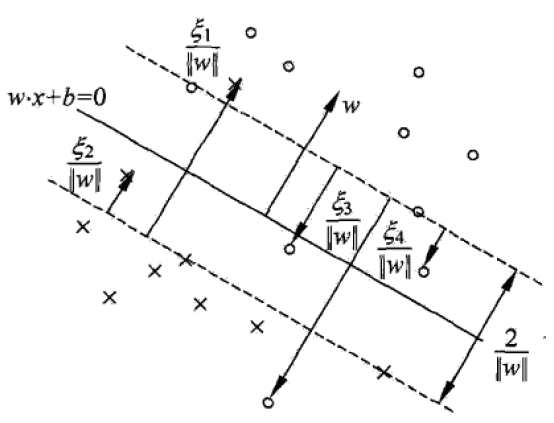
\includegraphics[height=5cm]{support}
\begin{itemize}
  \item If $\alpha_{i}^*<C$, we have $\xi=0$, support vectors $x_{i}$ is right on the margin boundary.
  \item If $\alpha_{i}^*=C$
        \begin{itemize}
          \item $0<\xi_{i}<1$, $x_{i}$ is correctly classified and between the separating hyperplane and margin boundary hyperplane.
          \item $\xi_{i}=1$, $x_{i}$ is right on the separating hyperplane.
          \item $\xi_{i}>1$, $x_{i}$ is wrongly classified.
        \end{itemize}
\end{itemize}

\section{Kernel methods}

\subsection{Nonlinearly separable case}
Generally speaking, we can't find a good linear classifier most of the time because dataset usually seems not to have a linear structure in real situation. In this section, we are trying to deal with nonlinearly separable case, which means that our dataset can be correctly classified by an $(N-1)$-dimensional hypersurface.\\
\\
Our main idea is to use a nonlinear mapping from input space to a feature space such that image set is approximately linearly separable in feature space. Here we give a simple example as the picture below.\\
\\
Suppose that input space (left picture) $\bm\chi\subset \mathbf{R^2},\ x=(x^{(1)},x^{(2)})^T\in \bm\chi$, image space $\bm Z\subset \mathbf{R^2},\ z=(z^{(1)},z^{(2)})^T\in \bm Z$.\\
Define a mapping $\bm\phi:\bm\chi\rightarrow\bm Z$ as:$$z=\bm\phi(x)=((x^{(1)})^2,(x^{(2)})^2)$$
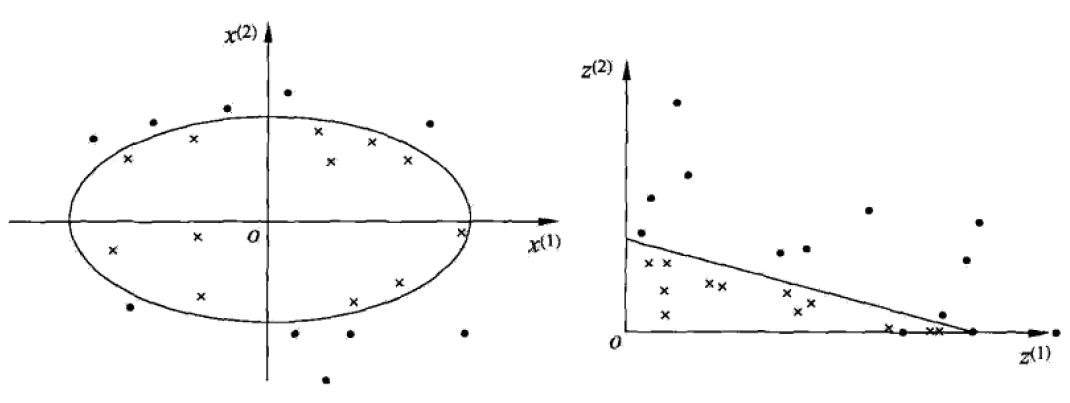
\includegraphics[width=10cm]{feature}\\
We can see that input space (left) can be separated by an ellipse $w_{1}(x^{(1)})^2+w_{2}(x^{(2)})^2+b=0$ which becomes a straight line $w_{1}z^{(1)}+w_{2}z^{(2)}+b=0$ after mapping to feature space (right). In this way, we transfer nonlinearly separable case in input space to linearly separable case in feature space.

\subsection{Kernel function}
We can see from the dual problem of linear SVM that either objective function or classifier decision function is only involved with inner product between input data points. When we use linear SVM in feature space, $x_{i}\cdot x_{j}$ is replaced by $\bm\phi(x_{i})\cdot \bm\phi(x_{j})$, which means we only need to concern the inner products between image points in feature space.\\

\paragraph{\textbf{Kernel function}} Suppose $\bm\chi$ is input space (subset of $\mathbf{R^n}$ or discrete set), $\mathscr{F}$ is feature space (Hilbert space), if there exists a mapping
$$\bm\phi:\bm\chi\rightarrow\mathscr{F}$$
such that for all $x,z\in \bm\chi$, function $k:\bm\chi\times\bm\chi\rightarrow\mathbf{R}$ satisfy:
$$k(x,z)=\bm\phi(x)\cdot\bm\phi(z)$$
Then we say $k(x,z)$ is a kernel function, $\bm\phi$ is a feature mapping.\\
\\
It's obvious that one feature mapping can only introduce one kernel function,but one kernel function may be able to be introduced by many different feature mappings. In real learning process, we only need to find proper kernel function instead of feature mapping. That's because on the one hand, the kernel function itself is enough to decide the final classifier; on the other hand, it's much easier and quicker to compute $k(x,z)$ than inner product $\bm\phi(x)\cdot\bm\phi(z)$ in $\mathscr{F}$ which is usually high-dimensional.\\

\paragraph{Gram matrix} Given a function $k:\bm\chi\times\bm\chi\rightarrow\mathbf{R}$ and inputs $x_{1},\cdots,x_{n}\in \bm\chi$, the $n\times n$ matrix
$$K:=(k(x_{i},x_{j}))_{ij}$$ is called the Gram matrix of k with respect to $x_{1},\cdots,x_{n}$.

\paragraph{Positive definite kernel} Let $\bm\chi$ be a nonempty set. A function $k:\bm\chi\times\bm\chi\rightarrow\mathbf{R}$ which for all $n\in \mathbf{N},\ x_{i}\in \bm\chi, i=1,\cdots,n$ gives rise to a positive definite Gram matrix is called a $positive\ definite\ kernel$.

\begin{theorem}
  A function $$k:\bm\chi\times\bm\chi\rightarrow\mathbf{R}$$ which is either continuous or has a finite domain, can be decomposed $$k(x,z)=\bm\phi(x)\cdot\bm\phi(z)$$
  into a feature map $\bm\phi$ into a Hilbert space $\mathscr{F}$ applied to both its arguments followed by the evaluation of the inner product in $\mathscr{F}$ if and only if it is a positive definite kernel.
\end{theorem}

\begin{proof}
 The 'only if' implication is trivial. We will mainly show the reverse implication.\\
 Assuming $k$ is a positive definite kernel, we'll proceed to construct a feature mapping $\bm\phi$ into a Hilbert space for which $k$ is the kernel.
 \begin{enumerate}
   \item Define the feature mapping $\bm\phi$ and construct a vector space $\bm F$.\\
      We define
      $$\bm\phi:x\longmapsto k(\bm x,\cdot)$$
      According to this mapping, we span the image set to a vector space
      $$\bm{F}=\{\sum_{i=1}^{l}\alpha_{i}k(\bm x_{i},\cdot):l\in\mathbf{N},\ \bm x_{i}\in\bm\chi,\ \alpha_{i}\in\mathbf{R},\ i=1,\cdots,N \}$$
   \item Make $\bm{F}$ an inner product space by defining inner product on $\bm F$.\\
      We define a binary function "$\bm{\cdot}$" on $\bm{F}$: for any $f,g\in \bm F$
      $$ f(\cdot)=\sum_{i=1}^{m}\alpha_{i}k(x_{i},\cdot) $$
      $$ g(\cdot)=\sum_{j=1}^{n}\beta_{i}k(x_{j},\cdot) $$
      $$ f\bm{\cdot} g=\sum_{i=1}^{m}\sum_{j=1}^{n}\alpha_{i}\beta_{j}k(x_{i},x_{j}) $$
      The bilinearity and symmetry are easy to prove. Now we show that this function is positive definite.
      $$ f\bm\cdot f=\sum_{i,j=1}^{m}\alpha_{i}\alpha_{j}k(x_{i},x_{j})=\alpha^T k\alpha $$
      Because the matrix K is positive semi-definite, we have $$f\bm\cdot f\geqslant 0,\ \forall\ f\in \bm{F}$$\\
      Utilizing this result, we can prove the Cauchy-Schwarz inequality
      \begin{equation}
        (f\bm\cdot g)^2\leqslant(f\bm\cdot f)(g\bm\cdot g)
      \end{equation}
      Notice that
      \begin{equation}
        f\bm\cdot k(x,\cdot)=\sum_{i=1}^{m}\alpha_{i}k(x_{i},x)=f(x)
      \end{equation}
      Take $g(\cdot)=K(x,\cdot)$ into (45), we have
      $$ (f\bm\cdot k(x,\cdot))^2=|f(x)|^2\leqslant(f\bm\cdot f)k(x,x) $$
      So while $f\bm\cdot f=0$, we have $f(x)\equiv 0$.
      Above all, binary function "$\bm\cdot$" satisfies bilinearity, symmetry and positive definiteness which means "$\bm\cdot$" is an inner product on $\bm{F}$. Now vector space $\bm{F}$ with inner product "$\bm\cdot$" is an inner product space.
   \item Complete the inner product space $\bm{F}$, we can get a Hilbert space $\mathscr{F}$.\\
      This Hilbert space is called $\textbf{reproducing\ kernel\ Hilbert\ space\ (RKHS)}$ because it satisfies equation (46) which is called $reproducing\ property$.
 \end{enumerate}
\end{proof}
\noindent\\
Back to SVM problem. When we choose a kernel function $K$, the objective function of dual problem turns out to be:
$$ W(\bm\alpha)=\frac{1}{2}\sum_{i=1}^{N}\sum_{j=1}^{N}\alpha_{i}\alpha_{j}y_{i}y_{j}-\sum_{i=1}^{N}\alpha_{i} $$
The decision function changes into:
$$ f(x)=sign(\ \sum_{i=1}^{N}\alpha_{i}^*y_{i}K(x_{i},x)+b^*\ ) $$

\subsection{Common kernel functions}
\begin{itemize}
  \item \textbf{Polynomial kernel function}:
        \begin{equation}
          K(\bm x,\bm z)=(\bm x\cdot \bm z+1)^{p}
        \end{equation}
  \item \textbf{Gaussian kernel function}
        \begin{equation}
          K(\bm x,\bm z)=exp(-\frac{\|\bm x-\bm z\|^2}{2\sigma^2})
        \end{equation}
  \item \textbf{sigmoid kernel function}
        \begin{equation}
          K(\bm x,\bm z)=tanh(\bm x\cdot \bm z+r)
        \end{equation}
\end{itemize}



%\end{document}
